% !TEX root = ../main.tex
\section{多层感知器简介}

多层感知器(Multilayer Perceptron, MLP)是一种前馈人工神经网络模型,是深度学习中最基本和常用的神经网络之一\cite{Goodfellow2016}。

\subsection{MLP的结构}

MLP通常由以下几个部分组成:
\begin{itemize}
    \item 输入层
    \item 一个或多个隐藏层
    \item 输出层
\end{itemize}

每一层都由多个神经元(或称为节点)组成,相邻层之间的神经元全连接。

\begin{figure}
    \centering
    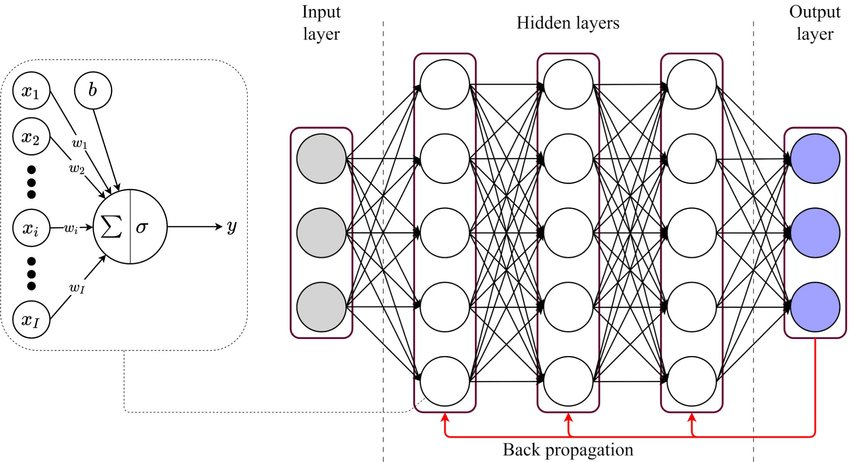
\includegraphics[width=0.8\textwidth]{mlp_structure.jpg}
    \caption{多层感知器的基本结构}
    \label{fig:mlp_structure}
\end{figure}

图~\ref{fig:mlp_structure}展示了一个典型的MLP结构。

\subsection{激活函数}

MLP中的每个神经元都使用非线性激活函数。常用的激活函数包括:

\begin{itemize}
    \item Sigmoid函数:$\sigma(x) = \frac{1}{1 + e^{-x}}$
    \item tanh函数:$\tanh(x) = \frac{e^x - e^{-x}}{e^x + e^{-x}}$
    \item ReLU函数:$ReLU(x) = \max(0, x)$
\end{itemize}

这些非线性激活函数使得MLP能够学习复杂的非线性映射关系\cite{Nair2010}。

\subsection{前向传播}

在MLP中,信息从输入层向前传播到输出层。对于一个具有一个隐藏层的MLP,其前向传播过程可以表示为:

\begin{equation}
    \mathbf{h} = f(\mathbf{W}_1\mathbf{x} + \mathbf{b}_1)
\end{equation}

\begin{equation}
    \mathbf{y} = g(\mathbf{W}_2\mathbf{h} + \mathbf{b}_2)
\end{equation}

其中,$\mathbf{x}$是输入,$\mathbf{h}$是隐藏层的输出,$\mathbf{y}$是最终输出,$\mathbf{W}_1$和$\mathbf{W}_2$是权重矩阵,$\mathbf{b}_1$和$\mathbf{b}_2$是偏置向量,$f$和$g$是激活函数。

更多关于神经网络的基础知识可以在斯坦福大学的CS231n课程网站上找到:\url{http://cs231n.stanford.edu/}
